\documentclass[12pt]{article}
\usepackage[utf8]{inputenc}
\usepackage{float}
\usepackage{amsmath}


\usepackage[hmargin=3cm,vmargin=6.0cm]{geometry}
%\topmargin=0cm
\topmargin=-2cm
\addtolength{\textheight}{6.5cm}
\addtolength{\textwidth}{2.0cm}
%\setlength{\leftmargin}{-5cm}
\setlength{\oddsidemargin}{0.0cm}
\setlength{\evensidemargin}{0.0cm}

%misc libraries goes here
\usepackage{tikz}
\usetikzlibrary{automata,positioning}

\begin{document}

\section*{Student Information } 
%Write your full name and id number between the colon and newline
%Put one empty space character after colon and before newline
Full Name : Nazır Bilal Yavuz \\
Id Number :  2099471\\

% Write your answers below the section tags
\section*{Answer 1}

\subsection*{a.}
It is countably infinite.\\ Lets think that there are only n rational numbers in the interval which is like\\
 \(c < r_1 < r_2  < r_3  < ... < r_n < d \)\\
 But there must be a rational in the interval \( c < r_1\), hence this is a contradiction and we can count them so this is a countably infinite.\\

\subsection*{b.}
By the definition of non regular languages, \( L^+ \) can not be finite and countable, so \(D \) is uncountable infinite set.\\

\subsection*{c.}
If the set is can not be recognized by Finite Automaton it must be non regular set so that it must be uncountable infinite set.
\\

\section*{Answer 2}

\subsection*{a.}
\begin{center}
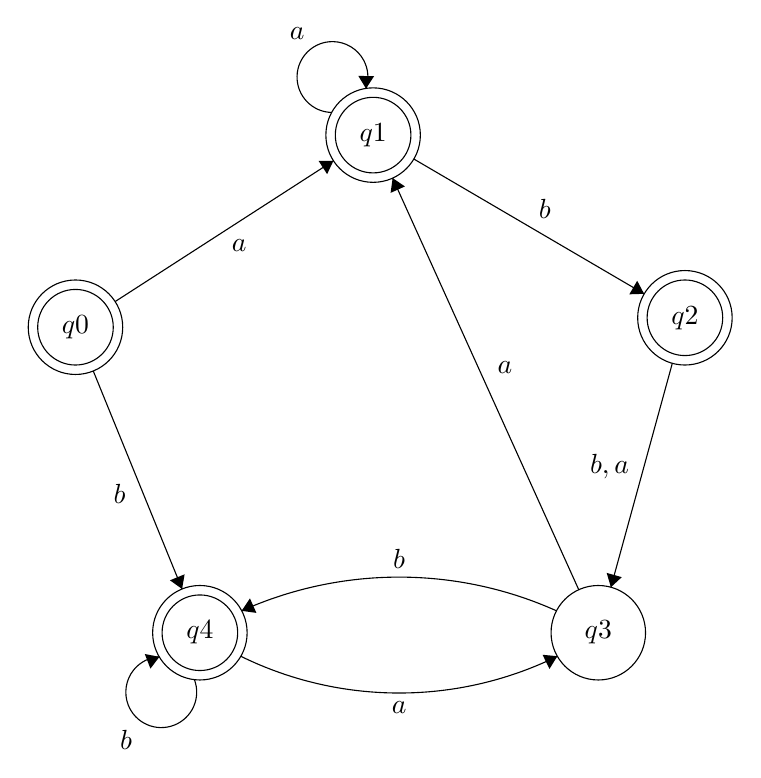
\begin{tikzpicture}[scale=0.2]
\tikzstyle{every node}+=[inner sep=0pt]
\draw [black] (15.2,-20.9) circle (3);
\draw (15.2,-20.9) node {$q0$};
\draw [black] (15.2,-20.9) circle (2.4);
\draw [black] (34.1,-8.7) circle (3);
\draw (34.1,-8.7) node {$q1$};
\draw [black] (34.1,-8.7) circle (2.4);
\draw [black] (53.9,-20.3) circle (3);
\draw (53.9,-20.3) node {$q2$};
\draw [black] (53.9,-20.3) circle (2.4);
\draw [black] (48.4,-40.3) circle (3);
\draw (48.4,-40.3) node {$q3$};
\draw [black] (23.1,-40.3) circle (3);
\draw (23.1,-40.3) node {$q4$};
\draw [black] (23.1,-40.3) circle (2.4);
\draw [black] (17.72,-19.27) -- (31.58,-10.33);
\fill [black] (31.58,-10.33) -- (30.64,-10.34) -- (31.18,-11.18);
\draw (25.59,-15.3) node [below] {$a$};
\draw [black] (36.69,-10.22) -- (51.31,-18.78);
\fill [black] (51.31,-18.78) -- (50.87,-17.95) -- (50.37,-18.81);
\draw (45,-14) node [above] {$b$};
\draw [black] (31.48,-7.263) arc (268.99202:-19.00798:2.25);
\draw (29.28,-2.67) node [above] {$a$};
\fill [black] (33.65,-5.75) -- (34.16,-4.96) -- (33.16,-4.94);
\draw [black] (53.1,-23.19) -- (49.2,-37.41);
\fill [black] (49.2,-37.41) -- (49.89,-36.77) -- (48.93,-36.5);
\draw (50.38,-29.77) node [left] {$b,a$};
\draw [black] (16.33,-23.68) -- (21.97,-37.52);
\fill [black] (21.97,-37.52) -- (22.13,-36.59) -- (21.2,-36.97);
\draw (18.41,-31.5) node [left] {$b$};
\draw [black] (45.801,-41.795) arc (-63.86028:-116.13972:22.815);
\fill [black] (45.8,-41.79) -- (44.86,-41.7) -- (45.3,-42.6);
\draw (35.75,-44.63) node [below] {$a$};
\draw [black] (22.748,-43.268) arc (20.97613:-267.02387:2.25);
\draw (18.42,-46.46) node [below] {$b$};
\fill [black] (20.53,-41.83) -- (19.6,-41.65) -- (19.96,-42.58);
\draw [black] (25.755,-38.907) arc (114.17109:65.82891:24.411);
\fill [black] (25.75,-38.91) -- (26.69,-39.04) -- (26.28,-38.12);
\draw (35.75,-36.27) node [above] {$b$};
\draw [black] (47.16,-37.57) -- (35.34,-11.43);
\fill [black] (35.34,-11.43) -- (35.21,-12.37) -- (36.12,-11.96);
\draw (41.97,-23.49) node [right] {$a$};
\end{tikzpicture}
\end{center}


\subsection*{b.}
\begin{center}
\begin{tikzpicture}[scale=0.2]
\tikzstyle{every node}+=[inner sep=0pt]
\draw [black] (35.8,-23.7) circle (3);
\draw (35.8,-23.7) node {$q0$};
\draw [black] (35.8,-23.7) circle (2.4);
\draw [black] (50.8,-23.7) circle (3);
\draw (50.8,-23.7) node {$q1$};
\draw [black] (48.9,-40.5) circle (3);
\draw (48.9,-40.5) node {$q2$};
\draw [black] (48.9,-40.5) circle (2.4);
\draw [black] (23.7,-45.8) circle (3);
\draw (23.7,-45.8) node {$q3$};
\draw [black] (67.1,-51.8) circle (3);
\draw (67.1,-51.8) node {$q6$};
\draw [black] (5,-36.1) circle (3);
\draw (5,-36.1) node {$q4$};
\draw [black] (5,-36.1) circle (2.4);
\draw [black] (12.9,-23.7) circle (3);
\draw (12.9,-23.7) node {$q5$};
\draw [black] (27.8,-14.8) circle (3);
\draw (27.8,-14.8) node {$q6$};
\draw [black] (27.8,-14.8) circle (2.4);
\draw [black] (38.8,-23.7) -- (47.8,-23.7);
\fill [black] (47.8,-23.7) -- (47,-23.2) -- (47,-24.2);
\draw (43.3,-24.2) node [below] {$a,b$};
\draw [black] (53.125,-25.574) arc (41.77558:-54.6805:9.188);
\fill [black] (51.59,-39.19) -- (52.53,-39.14) -- (51.95,-38.32);
\draw (56.06,-32.84) node [right] {$a,b$};
\draw [black] (46.871,-42.706) arc (-46.8679:-109.37771:20.115);
\fill [black] (26.45,-47) -- (27.03,-47.74) -- (27.37,-46.8);
\draw (37.86,-48.3) node [below] {$b$};
\draw [black] (51.45,-42.08) -- (64.55,-50.22);
\fill [black] (64.55,-50.22) -- (64.14,-49.37) -- (63.61,-50.22);
\draw (57.06,-46.65) node [below] {$a$};
\draw [black] (69.78,-50.477) arc (144:-144:2.25);
\draw (74.35,-51.8) node [right] {$a,b$};
\fill [black] (69.78,-53.12) -- (70.13,-54) -- (70.72,-53.19);
\draw [black] (69.78,-50.477) arc (144:-144:2.25);
\fill [black] (69.78,-53.12) -- (70.13,-54) -- (70.72,-53.19);
\draw [black] (21.04,-44.42) -- (7.66,-37.48);
\fill [black] (7.66,-37.48) -- (8.14,-38.29) -- (8.6,-37.41);
\draw (16.03,-40.44) node [above] {$a,b$};
\draw [black] (6.61,-33.57) -- (11.29,-26.23);
\fill [black] (11.29,-26.23) -- (10.44,-26.64) -- (11.28,-27.17);
\draw (9.57,-31.21) node [right] {$a,b$};
\draw [black] (14.097,-20.951) arc (153.66829:-28.47727:30.733);
\fill [black] (68.66,-49.24) -- (69.48,-48.77) -- (68.6,-48.3);
\draw (56.73,-6.8) node [above] {$a$};
\draw [black] (27.782,-17.787) arc (-9.53174:-108.76721:9.361);
\fill [black] (27.78,-17.79) -- (27.16,-18.49) -- (28.14,-18.66);
\draw (24.35,-24.77) node [below] {$b$};
\draw [black] (30.679,-13.97) arc (101.43297:36.25849:18.466);
\fill [black] (49.23,-21.15) -- (49.16,-20.21) -- (48.35,-20.8);
\draw (42.61,-14.31) node [above] {$a,b$};
\end{tikzpicture}
\end{center}

\subsection*{c.}
\begin{center}
\begin{tikzpicture}[scale=0.2]
\tikzstyle{every node}+=[inner sep=0pt]
\draw [black] (13.8,-42.4) circle (3);
\draw (13.8,-42.4) node {$q0$};
\draw [black] (13.8,-42.4) circle (2.4);
\draw [black] (49,-27) circle (3);
\draw (49,-27) node {$q1$};
\draw [black] (49,-27) circle (2.4);
\draw [black] (13.8,-9.2) circle (3);
\draw (13.8,-9.2) node {$q2$};
\draw [black] (72.5,-20.2) circle (3);
\draw (72.5,-20.2) node {$q3$};
\draw [black] (10.997,-41.364) arc (277.45184:-10.54816:2.25);
\draw (8.14,-37.02) node [above] {$b$};
\fill [black] (12.92,-39.55) -- (13.31,-38.69) -- (12.32,-38.82);
\draw [black] (47.539,-29.619) arc (-32.03328:-100.70797:29.824);
\fill [black] (47.54,-29.62) -- (46.69,-30.03) -- (47.54,-30.56);
\draw (35.13,-41.63) node [below] {$c$};
\draw [black] (13.8,-39.4) -- (13.8,-12.2);
\fill [black] (13.8,-12.2) -- (13.3,-13) -- (14.3,-13);
\draw (14.3,-25.8) node [right] {$a$};
\draw [black] (11.269,-7.611) arc (265.6075:-22.3925:2.25);
\draw (7.88,-2.95) node [above] {$a,b,c$};
\fill [black] (13.52,-6.22) -- (14.08,-5.47) -- (13.08,-5.39);
\draw [black] (15.214,-39.756) arc (148.92373:78.33503:29.173);
\fill [black] (15.21,-39.76) -- (16.05,-39.33) -- (15.2,-38.81);
\draw (27.53,-27.58) node [above] {$b$};
\draw [black] (51.88,-26.17) -- (69.62,-21.03);
\fill [black] (69.62,-21.03) -- (68.71,-20.78) -- (68.99,-21.74);
\draw (61.52,-24.15) node [below] {$a$};
\draw [black] (16.549,-7.999) arc (111.92076:46.85172:50.912);
\fill [black] (16.55,-8) -- (17.48,-8.16) -- (17.1,-7.24);
\draw (45.78,-4.54) node [above] {$a,c$};
\draw [black] (71.8,-23.116) arc (-15.82849:-122.73886:36.959);
\fill [black] (16.25,-44.12) -- (16.66,-44.98) -- (17.2,-44.14);
\draw (50.26,-48.13) node [below] {$b$};
\draw [black] (48.314,-24.092) arc (221.00538:-66.99462:2.25);
\draw (51.14,-19.85) node [above] {$c$};
\fill [black] (50.89,-24.69) -- (51.82,-24.54) -- (51.17,-23.78);
\end{tikzpicture}
\end{center}

\section*{Answer 3}

\begin{center}
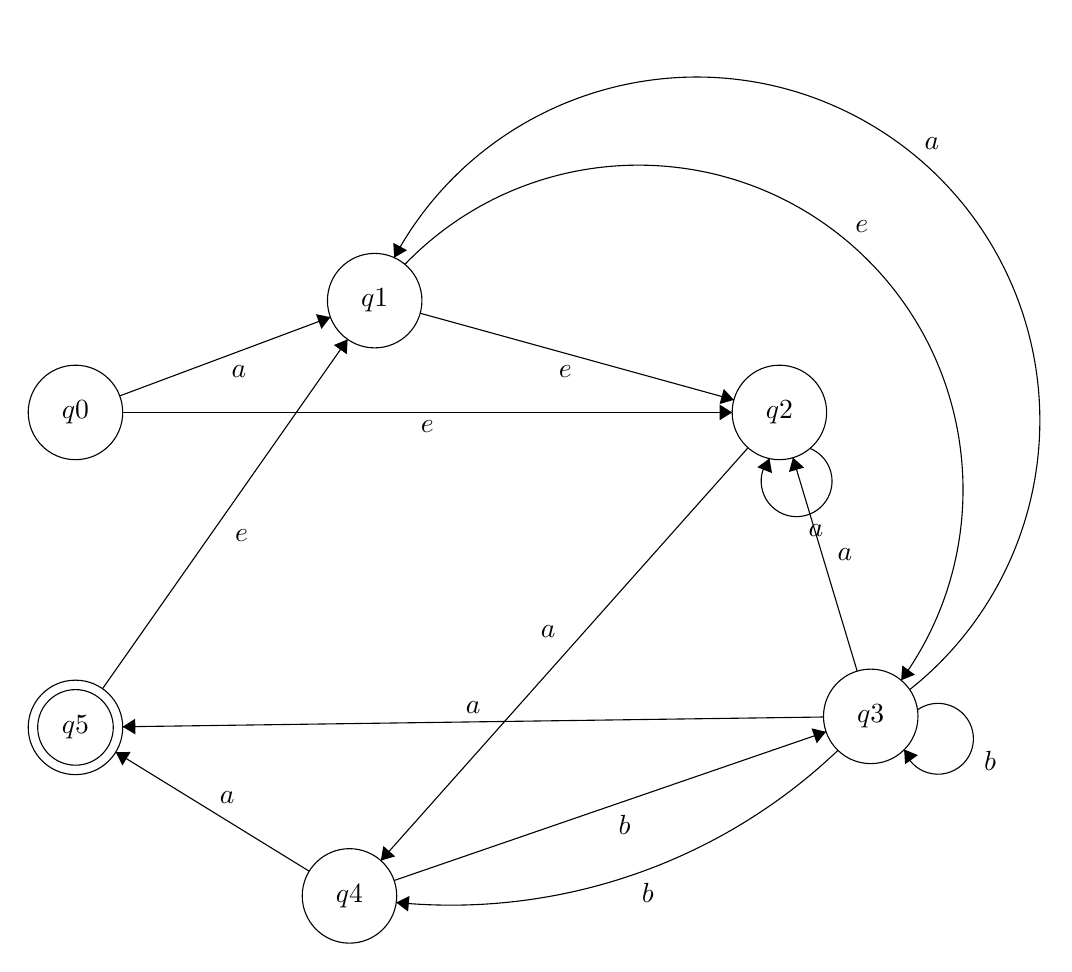
\begin{tikzpicture}[scale=0.2]
\tikzstyle{every node}+=[inner sep=0pt]
\draw [black] (12.5,-22.1) circle (3);
\draw (12.5,-22.1) node {$q0$};
\draw [black] (31.5,-15) circle (3);
\draw (31.5,-15) node {$q1$};
\draw [black] (57.2,-22.1) circle (3);
\draw (57.2,-22.1) node {$q2$};
\draw [black] (63,-41.4) circle (3);
\draw (63,-41.4) node {$q3$};
\draw [black] (29.9,-52.8) circle (3);
\draw (29.9,-52.8) node {$q4$};
\draw [black] (12.5,-42.1) circle (3);
\draw (12.5,-42.1) node {$q5$};
\draw [black] (12.5,-42.1) circle (2.4);
\draw [black] (15.5,-22.1) -- (54.2,-22.1);
\fill [black] (54.2,-22.1) -- (53.4,-21.6) -- (53.4,-22.6);
\draw (34.85,-22.6) node [below] {$e$};
\draw [black] (15.31,-21.05) -- (28.69,-16.05);
\fill [black] (28.69,-16.05) -- (27.77,-15.86) -- (28.12,-16.8);
\draw (22.88,-19.07) node [below] {$a$};
\draw [black] (34.39,-15.8) -- (54.31,-21.3);
\fill [black] (54.31,-21.3) -- (53.67,-20.61) -- (53.4,-21.57);
\draw (43.61,-19.11) node [below] {$e$};
\draw [black] (33.419,-12.697) arc (136.02935:-35.96178:20.609);
\fill [black] (64.93,-39.11) -- (65.81,-38.75) -- (65,-38.17);
\draw (62.44,-10.72) node [above] {$e$};
\draw [black] (59.133,-24.379) arc (68.03624:-219.96376:2.25);
\draw (59.52,-29.21) node [below] {$a$};
\fill [black] (56.57,-25.02) -- (55.8,-25.58) -- (56.73,-25.95);
\draw [black] (55.21,-24.34) -- (31.89,-50.56);
\fill [black] (31.89,-50.56) -- (32.8,-50.29) -- (32.05,-49.63);
\draw (43.01,-36) node [left] {$a$};
\draw [black] (32.737,-12.269) arc (151.68873:-51.62116:21.806);
\fill [black] (32.74,-12.27) -- (33.56,-11.8) -- (32.68,-11.33);
\draw (66.89,-5.41) node [above] {$a$};
\draw [black] (62.14,-38.53) -- (58.06,-24.97);
\fill [black] (58.06,-24.97) -- (57.81,-25.88) -- (58.77,-25.6);
\draw (60.87,-31.14) node [right] {$a$};
\draw [black] (60,-41.44) -- (15.5,-42.06);
\fill [black] (15.5,-42.06) -- (16.31,-42.55) -- (16.29,-41.55);
\draw (37.75,-41.24) node [above] {$a$};
\draw [black] (65.96,-40.993) arc (125.56505:-162.43495:2.25);
\draw (70.17,-44.24) node [right] {$b$};
\fill [black] (65.12,-43.5) -- (65.18,-44.44) -- (66,-43.86);
\draw [black] (60.917,-43.558) arc (-46.39049:-95.60098:35.623);
\fill [black] (32.87,-53.22) -- (33.62,-53.79) -- (33.71,-52.8);
\draw (48.85,-51.98) node [below] {$b$};
\draw [black] (27.34,-51.23) -- (15.06,-43.67);
\fill [black] (15.06,-43.67) -- (15.48,-44.52) -- (16,-43.66);
\draw (22.14,-46.95) node [above] {$a$};
\draw [black] (32.74,-51.82) -- (60.16,-42.38);
\fill [black] (60.16,-42.38) -- (59.24,-42.16) -- (59.57,-43.11);
\draw (47.36,-47.63) node [below] {$b$};
\draw [black] (14.22,-39.64) -- (29.78,-17.46);
\fill [black] (29.78,-17.46) -- (28.91,-17.82) -- (29.73,-18.4);
\draw (22.6,-29.91) node [right] {$e$};
\end{tikzpicture}
\end{center}
\subsection*{a.}
We can only reach \( q_5 \) with an \textit{a}. They are \( q_4 \rightarrow q_5 \) and \( q_3 \rightarrow q_5 \). So that \textit{abbb} is not reachable.

\subsection*{b.}
For \textit{w = ababa} we can trace \( q_0 \rightarrow q_1 \rightarrow q_3 \rightarrow q_3 \rightarrow q_5 \rightarrow q_1 \rightarrow q_3 \rightarrow q_3 \rightarrow q_5\).\\




\section*{Answer 4}

\begin{center}
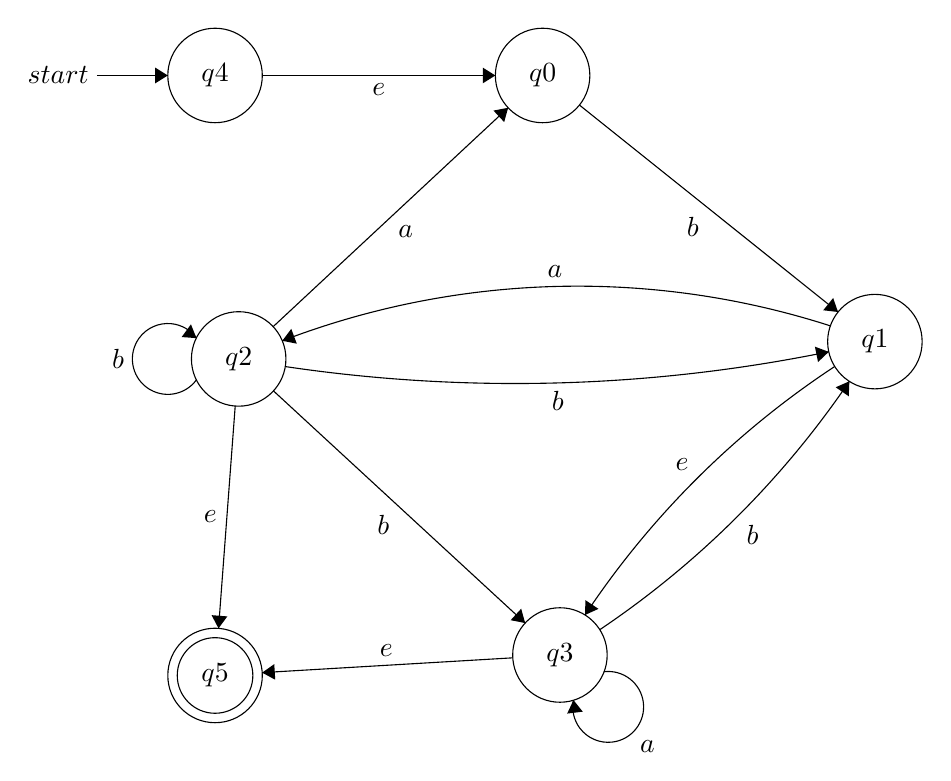
\begin{tikzpicture}[scale=0.2]
\tikzstyle{every node}+=[inner sep=0pt]
\draw [black] (35,-11.6) circle (3);
\draw (35,-11.6) node {$q0$};
\draw [black] (56.1,-28.5) circle (3);
\draw (56.1,-28.5) node {$q1$};
\draw [black] (15.7,-29.6) circle (3);
\draw (15.7,-29.6) node {$q2$};
\draw [black] (36.1,-48.4) circle (3);
\draw (36.1,-48.4) node {$q3$};
\draw [black] (14.2,-11.6) circle (3);
\draw (14.2,-11.6) node {$q4$};
\draw [black] (14.2,-49.7) circle (3);
\draw (14.2,-49.7) node {$q5$};
\draw [black] (14.2,-49.7) circle (2.4);
\draw [black] (37.34,-13.48) -- (53.76,-26.62);
\fill [black] (53.76,-26.62) -- (53.45,-25.73) -- (52.82,-26.51);
\draw (44.54,-20.54) node [below] {$b$};
\draw [black] (18.469,-28.447) arc (110.96982:72.14947:52.382);
\fill [black] (18.47,-28.45) -- (19.39,-28.63) -- (19.04,-27.69);
\draw (35.78,-24.47) node [above] {$a$};
\draw [black] (37.693,-45.858) arc (146.38101:123.3318:55.983);
\fill [black] (37.69,-45.86) -- (38.55,-45.47) -- (37.72,-44.92);
\draw (43.86,-36.69) node [above] {$e$};
\draw [black] (17.89,-27.55) -- (32.81,-13.65);
\fill [black] (32.81,-13.65) -- (31.88,-13.83) -- (32.56,-14.56);
\draw (26.31,-21.08) node [below] {$a$};
\draw [black] (53.17,-29.145) arc (-78.43985:-98.44085:99.399);
\fill [black] (53.17,-29.15) -- (52.29,-28.82) -- (52.49,-29.8);
\draw (35.97,-31.65) node [below] {$b$};
\draw [black] (13.02,-30.923) arc (324:36:2.25);
\draw (8.45,-29.6) node [left] {$b$};
\fill [black] (13.02,-28.28) -- (12.67,-27.4) -- (12.08,-28.21);
\draw [black] (17.91,-31.63) -- (33.89,-46.37);
\fill [black] (33.89,-46.37) -- (33.64,-45.46) -- (32.97,-46.19);
\draw (24.88,-39.49) node [below] {$b$};
\draw [black] (54.478,-31.023) arc (-34.19454:-56.09265:58.847);
\fill [black] (54.48,-31.02) -- (53.61,-31.4) -- (54.44,-31.97);
\draw (48.33,-40.14) node [below] {$b$};
\draw [black] (38.893,-49.462) arc (96.90714:-191.09286:2.25);
\draw (41.66,-53.83) node [below] {$a$};
\fill [black] (36.96,-51.26) -- (36.56,-52.12) -- (37.55,-52);
\draw [black] (17.2,-11.6) -- (32,-11.6);
\fill [black] (32,-11.6) -- (31.2,-11.1) -- (31.2,-12.1);
\draw (24.6,-12.1) node [below] {$e$};
\draw [black] (6.7,-11.6) -- (11.2,-11.6);
\draw (6.2,-11.6) node [left] {$start$};
\fill [black] (11.2,-11.6) -- (10.4,-11.1) -- (10.4,-12.1);
\draw [black] (15.48,-32.59) -- (14.42,-46.71);
\fill [black] (14.42,-46.71) -- (14.98,-45.95) -- (13.98,-45.87);
\draw (14.34,-39.6) node [left] {$e$};
\draw [black] (33.11,-48.58) -- (17.19,-49.52);
\fill [black] (17.19,-49.52) -- (18.02,-49.97) -- (17.96,-48.98);
\draw (25.08,-48.5) node [above] {$e$};
\end{tikzpicture}
\end{center}

\subsection*{b.}

Eliminate \(q_0\)

\begin{center}
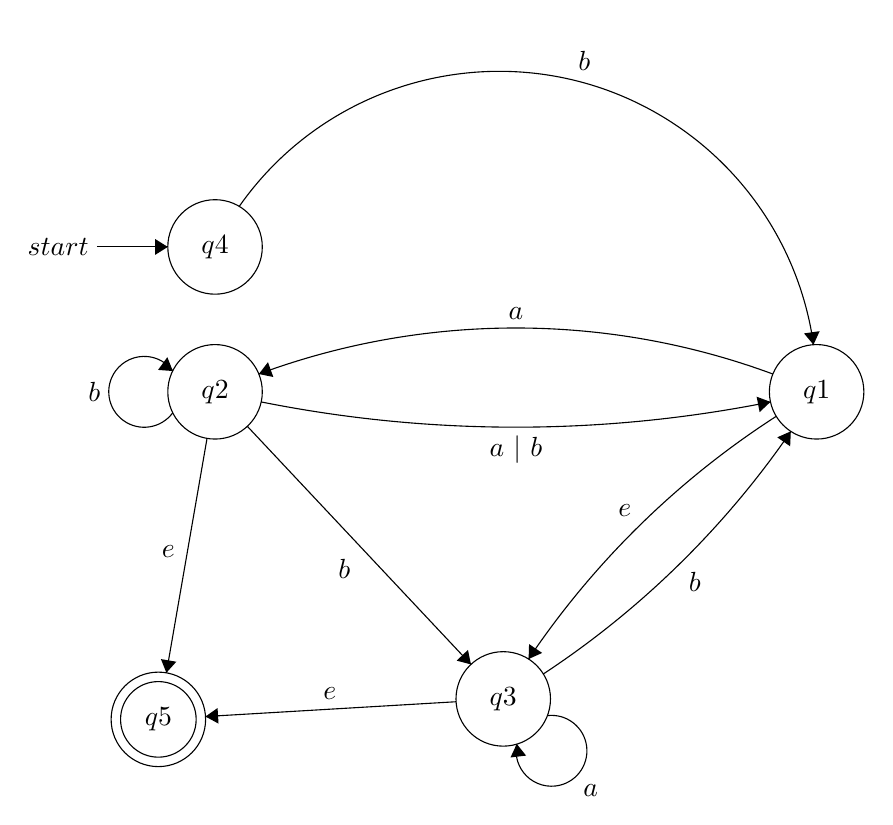
\begin{tikzpicture}[scale=0.2]
\tikzstyle{every node}+=[inner sep=0pt]
\draw [black] (56,-28.9) circle (3);
\draw (56,-28.9) node {$q1$};
\draw [black] (17.8,-28.9) circle (3);
\draw (17.8,-28.9) node {$q2$};
\draw [black] (36.1,-48.4) circle (3);
\draw (36.1,-48.4) node {$q3$};
\draw [black] (17.8,-19.7) circle (3);
\draw (17.8,-19.7) node {$q4$};
\draw [black] (14.2,-49.7) circle (3);
\draw (14.2,-49.7) node {$q5$};
\draw [black] (14.2,-49.7) circle (2.4);
\draw [black] (20.578,-27.77) arc (110.31062:69.68938:47.022);
\fill [black] (20.58,-27.77) -- (21.5,-27.96) -- (21.16,-27.02);
\draw (36.9,-24.35) node [above] {$a$};
\draw [black] (37.706,-45.867) arc (146.04858:122.78809:54.616);
\fill [black] (37.71,-45.87) -- (38.57,-45.48) -- (37.74,-44.92);
\draw (43.82,-36.88) node [above] {$e$};
\draw [black] (53.07,-29.543) arc (-78.67535:-101.32465:82.344);
\fill [black] (53.07,-29.54) -- (52.19,-29.21) -- (52.38,-30.19);
\draw (36.9,-31.65) node [below] {$a\mbox{ }|\mbox{ }b$};
\draw [black] (15.12,-30.223) arc (324:36:2.25);
\draw (10.55,-28.9) node [left] {$b$};
\fill [black] (15.12,-27.58) -- (14.77,-26.7) -- (14.18,-27.51);
\draw [black] (19.85,-31.09) -- (34.05,-46.21);
\fill [black] (34.05,-46.21) -- (33.86,-45.29) -- (33.14,-45.97);
\draw (26.42,-40.12) node [left] {$b$};
\draw [black] (54.365,-31.415) arc (-34.53223:-56.63109:57.409);
\fill [black] (54.36,-31.41) -- (53.5,-31.79) -- (54.32,-32.36);
\draw (48.27,-40.35) node [below] {$b$};
\draw [black] (38.893,-49.462) arc (96.90714:-191.09286:2.25);
\draw (41.66,-53.83) node [below] {$a$};
\fill [black] (36.96,-51.26) -- (36.56,-52.12) -- (37.55,-52);
\draw [black] (10.3,-19.7) -- (14.8,-19.7);
\draw (9.8,-19.7) node [left] {$start$};
\fill [black] (14.8,-19.7) -- (14,-19.2) -- (14,-20.2);
\draw [black] (17.29,-31.86) -- (14.71,-46.74);
\fill [black] (14.71,-46.74) -- (15.34,-46.04) -- (14.36,-45.87);
\draw (15.28,-39.06) node [left] {$e$};
\draw [black] (33.11,-48.58) -- (17.19,-49.52);
\fill [black] (17.19,-49.52) -- (18.02,-49.97) -- (17.96,-48.98);
\draw (25.08,-48.5) node [above] {$e$};
\draw [black] (19.335,-17.126) arc (144.92444:7.99334:20.164);
\fill [black] (55.8,-25.91) -- (56.19,-25.05) -- (55.2,-25.19);
\draw (41.25,-8.54) node [above] {$b$};
\end{tikzpicture}
\end{center}

Eliminate \(q_3\)

\begin{center}
\begin{tikzpicture}[scale=0.2]
\tikzstyle{every node}+=[inner sep=0pt]
\draw [black] (56,-28.9) circle (3);
\draw (56,-28.9) node {$q1$};
\draw [black] (17.8,-28.9) circle (3);
\draw (17.8,-28.9) node {$q2$};
\draw [black] (17.8,-19.7) circle (3);
\draw (17.8,-19.7) node {$q4$};
\draw [black] (14.2,-49.7) circle (3);
\draw (14.2,-49.7) node {$q5$};
\draw [black] (14.2,-49.7) circle (2.4);
\draw [black] (20.578,-27.77) arc (110.31062:69.68938:47.022);
\fill [black] (20.58,-27.77) -- (21.5,-27.96) -- (21.16,-27.02);
\draw (36.9,-24.35) node [above] {$a$};
\draw [black] (53.07,-29.543) arc (-78.67535:-101.32465:82.344);
\fill [black] (53.07,-29.54) -- (52.19,-29.21) -- (52.38,-30.19);
\draw (36.9,-31.65) node [below] {$a\mbox{ }|\mbox{ }b\mbox{ }|\mbox{ }(ba*b)$};
\draw [black] (15.12,-30.223) arc (324:36:2.25);
\draw (10.55,-28.9) node [left] {$b$};
\fill [black] (15.12,-27.58) -- (14.77,-26.7) -- (14.18,-27.51);
\draw [black] (10.3,-19.7) -- (14.8,-19.7);
\draw (9.8,-19.7) node [left] {$start$};
\fill [black] (14.8,-19.7) -- (14,-19.2) -- (14,-20.2);
\draw [black] (17.29,-31.86) -- (14.71,-46.74);
\fill [black] (14.71,-46.74) -- (15.34,-46.04) -- (14.36,-45.87);
\draw (15.28,-39.06) node [left] {$e\mbox{ }|\mbox{ }(ba*)$};
\draw [black] (19.335,-17.126) arc (144.92444:7.99334:20.164);
\fill [black] (55.8,-25.91) -- (56.19,-25.05) -- (55.2,-25.19);
\draw (41.25,-8.54) node [above] {$b$};
\draw [black] (54.205,-31.303) arc (-38.51398:-88.57544:48.846);
\fill [black] (17.2,-49.72) -- (18.01,-50.2) -- (17.99,-49.2);
\draw (39.18,-45.12) node [below] {$a*$};
\end{tikzpicture}
\end{center}

Eliminate \( q_1 \)

\begin{center}
\begin{tikzpicture}[scale=0.2]
\tikzstyle{every node}+=[inner sep=0pt]
\draw [black] (63.7,-23.1) circle (3);
\draw (63.7,-23.1) node {$q2$};
\draw [black] (20.7,-12.9) circle (3);
\draw (20.7,-12.9) node {$q4$};
\draw [black] (14.2,-49.7) circle (3);
\draw (14.2,-49.7) node {$q5$};
\draw [black] (14.2,-49.7) circle (2.4);
\draw [black] (64.26,-20.165) arc (196.93075:-91.06925:2.25);
\draw (68.77,-17.22) node [above] {$b$};
\fill [black] (66.37,-21.76) -- (67.28,-22) -- (66.99,-21.05);
\draw [black] (13.2,-12.9) -- (17.7,-12.9);
\draw (12.7,-12.9) node [left] {$start$};
\fill [black] (17.7,-12.9) -- (16.9,-12.4) -- (16.9,-13.4);
\draw [black] (61.61,-25.252) arc (-45.14699:-78.34818:88.336);
\fill [black] (17.15,-49.14) -- (18.03,-49.47) -- (17.83,-48.49);
\draw (44.86,-40.95) node [below] {$e\mbox{ }|\mbox{ }(ba*)$};
\draw [black] (23.62,-13.59) -- (60.78,-22.41);
\fill [black] (60.78,-22.41) -- (60.12,-21.74) -- (59.89,-22.71);
\draw (49.14,-16.74) node [above] {$ba\mbox{ }|\mbox{ }(bab*a\mbox{ }|\mbox{ }b\mbox{ }|\mbox{ }(ba*b)a)$};
\draw [black] (20.18,-15.85) -- (14.72,-46.75);
\fill [black] (14.72,-46.75) -- (15.35,-46.04) -- (14.37,-45.87);
\draw (18.17,-31.55) node [right] {$ba*\mbox{ }|\mbox{ }(bab*a\mbox{ }|\mbox{ }b\mbox{ }|\mbox{ }(ba*b)a*)$};
\end{tikzpicture}
\end{center}

Eliminate \(q_2\)

\begin{center}
\begin{tikzpicture}[scale=0.2]
\tikzstyle{every node}+=[inner sep=0pt]
\draw [black] (20.7,-12.9) circle (3);
\draw (20.7,-12.9) node {$q4$};
\draw [black] (15.3,-43.8) circle (3);
\draw (15.3,-43.8) node {$q5$};
\draw [black] (15.3,-43.8) circle (2.4);
\draw [black] (13.2,-12.9) -- (17.7,-12.9);
\draw (12.7,-12.9) node [left] {$start$};
\fill [black] (17.7,-12.9) -- (16.9,-12.4) -- (16.9,-13.4);
\draw [black] (20.18,-15.86) -- (15.82,-40.84);
\fill [black] (15.82,-40.84) -- (16.45,-40.14) -- (15.46,-39.97);
\draw (18.72,-28.6) node [right] {$ba*|\mbox{ }(bab*a\mbox{ }|\mbox{ }b\mbox{ }|\mbox{ }(ba*b)a*)\mbox{ }|\mbox{ }(e\mbox{ }|\mbox{ }(ba*))$};
\end{tikzpicture}
\end{center}




\section*{Answer 5}

\subsection*{a.}

\begin{table}[htb]
\centering
\caption{Transition Table}
\label{my-label}
\begin{tabular}{|l|l|l|l}
\cline{1-3}
               & a          & b      &  \\ \cline{1-3}
\{q0, q1 ,q2\} & \{q1,q3\}  & \{q2\} &  \\ \cline{1-3}
\{q1, q3\}     &  $\O$          & \{q1\} &  \\ \cline{1-3}
\{q2\}         & \{q1, q3\} &  $\O$      &  \\ \cline{1-3}
\{q1\}         &    $\O$        &  $\O$      &  \\ \cline{1-3}
\end{tabular}
\end{table}

\begin{center}
\begin{tikzpicture}[scale=0.2]
\tikzstyle{every node}+=[inner sep=0pt]
\draw [black] (17.9,-14.8) circle (3);
\draw (17.9,-14.8) node {${q_0,\mbox{ }q_1,\mbox{ }q_2}$};
\draw [black] (17.9,-48.9) circle (3);
\draw (17.9,-48.9) node {$q_2$};
\draw [black] (51.6,-14.8) circle (3);
\draw (51.6,-14.8) node {$q_1$};
\draw [black] (42.6,-35.6) circle (3);
\draw (42.6,-35.6) node {${q_1,\mbox{ }q_3}$};
\draw [black] (55.9,-48.9) circle (3);
\draw [black] (20.19,-16.73) -- (40.31,-33.67);
\fill [black] (40.31,-33.67) -- (40.02,-32.77) -- (39.37,-33.53);
\draw (29.3,-25.69) node [below] {$a$};
\draw [black] (17.9,-17.8) -- (17.9,-45.9);
\fill [black] (17.9,-45.9) -- (18.4,-45.1) -- (17.4,-45.1);
\draw (17.4,-31.85) node [left] {$b$};
\draw [black] (43.79,-32.85) -- (50.41,-17.55);
\fill [black] (50.41,-17.55) -- (49.63,-18.09) -- (50.55,-18.49);
\draw (47.83,-26.16) node [right] {$b$};
\draw [black] (20.54,-47.48) -- (39.96,-37.02);
\fill [black] (39.96,-37.02) -- (39.02,-36.96) -- (39.49,-37.84);
\draw (31.19,-42.75) node [below] {$a$};
\draw [black] (20.9,-48.9) -- (52.9,-48.9);
\fill [black] (52.9,-48.9) -- (52.1,-48.4) -- (52.1,-49.4);
\draw (36.9,-49.4) node [below] {$b$};
\draw [black] (54.567,-15.217) arc (77.08788:-62.71379:17.464);
\fill [black] (58.67,-47.76) -- (59.61,-47.84) -- (59.15,-46.95);
\draw (68.66,-29.92) node [right] {$a,b$};
\draw [black] (44.72,-37.72) -- (53.78,-46.78);
\fill [black] (53.78,-46.78) -- (53.57,-45.86) -- (52.86,-46.57);
\draw (48.28,-42.73) node [below] {$a$};
\end{tikzpicture}
\end{center}

\subsection*{b.}

We can figure out that:\\ 
\(L(N) = a | ba\) so that,\\
$\overline{L}$\((N) = \{a,b\}^* - a | ba\)
\section*{Answer 6}
\(L_1\) and \(L_2\) is regular expression and we know that \(L_1\) - \(L_2\) is also regular but we must prove that by constructing \(NFA\).\\
1- Change the expression: \(L_1\) - \(L_2\)  = \(L_1\) $\cap$ $\overline{L_2}$\\
2- We can use method which we used in Question 4 part A.\\
3- When we using method $\overline{L_2}$ we must change the arrows' directions.\\
4- After that we must use intersection operation on \(NFA\).
5- Now the expression is = \(L_1\) $\cap$ $\overline{L_2}$ which is equal to \(L_1\) - \(L_2\).\\
6- We can use this algorithm.\\ 


\section*{Answer 7}

\subsection*{a.}
Lets assume \(w = aaaaaaaaa\)\\ 
And \(x = aaaa\), \(y = aa\) and \(z = aaa\).\\ 
Lets take \(xy^2z\) which is equal to \(aaaaaaaaaaa\)\\ Hence, number of \(a\)'s are \(11\) so this is not a regular.




\end{document}

​

